\chapter[敏捷开发]{再读XY理论:如何支持敏捷开发}

培训一开始,我把3天的范围、敏捷的主要概念讲完后,立即在白板左右两面写上一些数据,让学员猜它们分别是美国西岸哪两家科网公司?

``大家猜一下,下面两家都是美国西岸的公司分别是什么公司?''\\
我在敏捷ACP 培训,通常都会用这个问题开头。\\

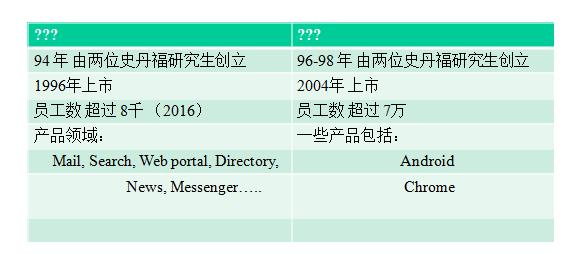
\includegraphics[width=10cm]{0A_Agile_stories_p4.jpg}

他们立即猜到左面是 YAHOO! , 右面是Google 。\\
2000年,谷歌还是小公司,雅虎是已经是大规模的上市公司,但现在大部分人只认识谷歌,原因是雅虎已经在2017年被收购
(虽然品牌还在),但反过来,谷歌公司从本来2000年的一个小公司,变成目前全球IT界举足轻重的超级大公司。\\
他们两家公司有什么区分呢?为什么是这样的结果呢?\\

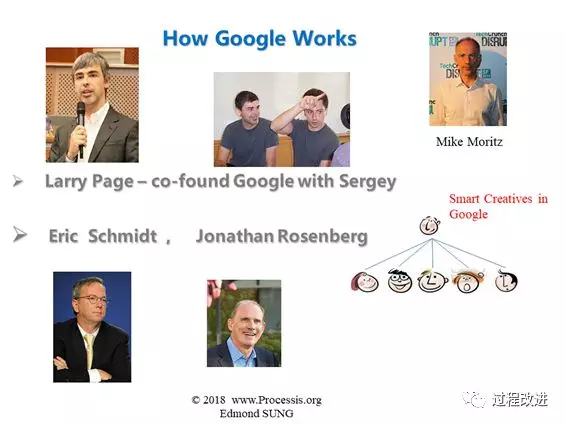
\includegraphics[width=10cm]{香港敏捷2.jpg}

接下来,我会借用谷歌的实例,说明敏捷的原则。\\
Eric本来是NOVELL的CEO,2002年加入了谷歌当CEO。第一天进办公室的时候,他发现风格跟其他东岸的公司完全不一样,例如他的办公室不大。过了一两天以后,竟然有个工程师走过来说:``我们那边太挤了,我看你那边还是挺宽松,我可否搬到你这边来?''\\
"为什么一个工程师还可以进CEO的办公室占位置?"\\
Eric虽然心里觉得很奇怪,
但新来公司,不熟悉谷歌的文化,他便回答:好的,欢迎,没问题。\\
谷歌是有两位斯坦福的研究生创立的,可能大家都知道它是以搜索引擎起家,虽然小,但是技术很厉害。所以开始被当时的巨无霸微软看成是下一个攻击和收购的目标。微软擅长用各种手段打击竞争对手,以垄断市场方面。

董事会的Mike 就发邮件提醒他要准备应对微软的策略
(微软会对有威胁的新公司极力打击)。\\
Eric进了公司后不久,创始人Larry
Page也聘用了另外一个很资深的管理者Jonathan,所以Jonathan和Eric就担起这个任务,要做一个应对微软的计划书,他们都是职场老手,有很资深的商业经验,他们就用传统的方式做了一个详细的业务计划书,计划在未来两年时间如何部署、准备。
计划书很详细,有很多数字支撑。\\
Jonathan很有经验,觉得这个计划还是挺完备的,就拿给创始人Larry看,Eric也在场。\\
Larry 看了几分钟后就问Jonathan:以前试过你们的团队超越了你的计划吗?\\
Larry看Jonathan和Eric好像不太理解,继续说:你见过哪个团队的表现能超越既定目标?你的团队研发过比计划中更出色的产品吗?\\
Jonathan 和 Eric都无法回答。\\
Larry说:如果是这样,计划还有什么意义?\\
最后Larry说一定还有比计划更有效的方式,于是让他们去和工程师谈谈。
他们便发现Google公司的工程师都是既有技术能力,也很有商业头脑的创意精英
(Smart Creative),不需要用硬性的计划来推动。计划反而会妨碍他们的创意。\\
这故事让学员知道要敏捷必须具备一些基本条件:敏捷不是一个万应万灵的魔术棒,不是照着去做便会敏捷成功。\\
另一方面 YAHOO 上市后 便有了各样的 ``大公司''病 ------
官僚化的管理,导致最终被收购。

比如在Google的一些内部讨论中,做决定不只是依据提出者的公司地位、权力,
一些由高管提出的意见不足同样可以被工程师推翻
,Google叫这些横行的管理者为河马(HiPPO : Highest-Paid Person's Opinion)
, 下午做活动练习时 不少组员 常常提到自己公司确实有不少河马在横行。

\hypertarget{ux7f8eux56fdux8d39ux57ce-weisbordux6545ux4e8b}{%
\subsection{美国费城
Weisbord故事}\label{ux7f8eux56fdux8d39ux57ce-weisbordux6545ux4e8b}}

X-Y理论能让我们更理解敏捷开发的原则,每当一些敏捷ACP班学员质疑捷开发是否确实能提升团队的生产率,我就会用
以下故事,让他们感受如何让团队自主管理的过程:

60年代, 复印机还未普及,很昂贵,所以为各类公司客户提供印刷服务有市场,
这故事的主人翁是某美国东岸一家印刷公司的老板儿子Weisbord。
他一直都没有接受什么正式的管理培训。 他有一个好朋友 Don
在国际大公司已工作了20年,
Don推荐Weisbord说:``很多大公司已经开始推进团队自主管理,提升生产率,
你可以先读 X-Y理论 (McGregor `Human side of Enterprise')一书``

X理论:\\

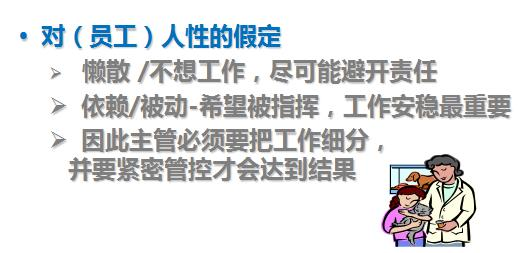
\includegraphics[width=10cm]{0A_Agile_stories_p2.jpg}\\

Y理论:\\

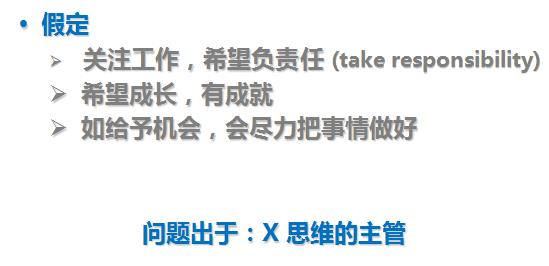
\includegraphics[width=6cm]{0A_Agile_stories_p3.jpg}\\
Weisbord本来只想看看有多厉害,但他结果一口气一周末读完全书。他发现自己公司到处都是都是X理论管理:\\

\begin{itemize}
\tightlist
\item
  工作分得很细,每员工不清楚全局
\item
  任务都是依赖主管分配
\item
  员工遇到问题、困难,交给主管处理
\item
  员工上下班打卡
\end{itemize}

他觉得这方式应该可以帮公司提升,但他担心但靠自己推动不了这个改革,
他便请Don过来正式加入公司。

他们分析公司业务最大问题是订单处理部门(Order Processing),
每个订单处理工作分到五、六个任务,员工只管被分配的任务,例如:

\begin{itemize}
\tightlist
\item
  筛选客户邮寄地址,邮寄印刷样本
\item
  输入订单
\item
  检查客户的信用
\item
  发起内部生产订单
\item
  用打字机打发票邮寄出去
\item
  收到的支票,对上那些应付账
\end{itemize}

公司平均每天要处理200到300个订单,
但因为工作分得很细,如果某个任务(如输入订单)有一、两人缺席,
便严重影响整个流程,效率会降低一半。

针对这问题,Weisbord 计划改革,把这部门的人分成多个4-5人团队,
把公司的两万个客户按地区分到各团队,每个团队有自己的客户名单,打字机等设备,
希望可以增加部门的灵活度和生产率。

Weisbord与5位小主管(supervisor)商量,2位很赞成,2位中立,其他1位觉得不会成功。
Weisbord决策启动这改革,与Don开始重组部门。

\hypertarget{ux5f00ux59cbux56e2ux961fux5236}{%
\subsubsection{开始团队制}\label{ux5f00ux59cbux56e2ux961fux5236}}

开始时问题非常多:

\begin{itemize}
\tightlist
\item
  B物流公司运送出错,送到另一个城市,怎么办?
\item
  D团队误解了生产的步骤,怎么办?
\item
  C团队的样板工人,刚入职3周,对我们公司产品线不熟识,怎么办?
\end{itemize}

原因很简单:本来每个人以前都只懂自己的一小块工作,以前问题都是由小主管处理。现在自主团队没有主管,都要靠团队自己想办法,像瞎子摸象。

但问题确实太多了,没办法,Don建议每周开会讨论。
他们从未有每周开会的习惯,Weisbord本来以为开会浪费时间,把时间用于生产更实际。
问题一直都非常多,延续了一个月

Weisbord开始怀疑这X-Y理论,只是大学象牙塔里的玩意,难以真正用于实际公司环境。
Don也没有更好的建议。

Weisbord开始有撤销整个改革的想法,返回本来的组织架构,
Don还希望Weisbord稍等一两周,看看有没有好转。但Weisbord觉得一直这么多问题,严重影响公司运作,也难以与父亲交代,想在下次开会时向大家宣布变回本来架构。

到了第五周开会:\\
Weisbord,与以前开会一样,先问: 大家有什么问题?\\
沉默,几分钟后,某组长说:没有问题。\\
Weisbord: 为什么会没有?一直这么多问题\\
:(心里想,一定是你们也放弃了,连问题都不愿提了。)\\
另一组长回答:我们今周没有什么问题,遇到的问题都在以前的会议里面被解决了。\\

\hypertarget{ux6548ux679c}{%
\subsubsection{效果}\label{ux6548ux679c}}

改革的后果中本来低于每天一天300个订单提升到400。
员工出勤率也改善,缺席率也降低到接近零。

改革后的订单处理部平面图: 

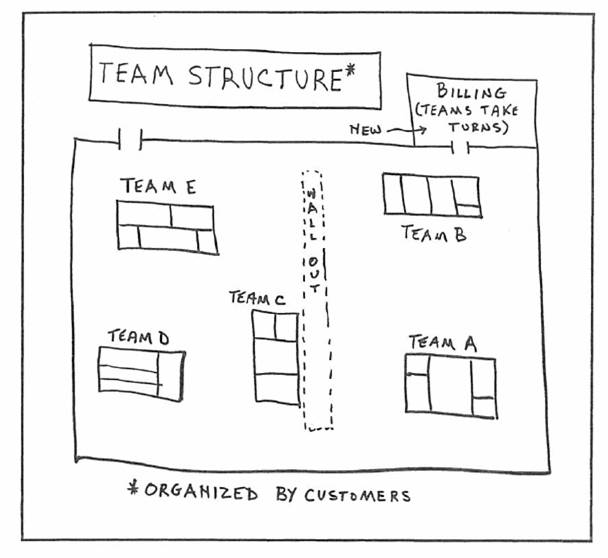
\includegraphics[width=10cm]{0A_Agile_stories_p5.jpg}

(团队自主改革前,小主管们为了减少各功能之间在处理订单引起的争吵,特意在中间加了一道墙;后面团队们一致建议把墙拆掉。)

Weisbord事后回顾:所有改变,重组都需要时间磨合,过程中管理者的支持非常重要,如果管理者不能坚持,面对并解决面对的困难,便会以失败告终。

\hypertarget{google-ux4e0e-weisbord-ux6545ux4e8bux7684ux542fux53d1}{%
\subsection{Google 与 Weisbord
故事的启发}\label{google-ux4e0e-weisbord-ux6545ux4e8bux7684ux542fux53d1}}

如果员工具备知能,管理者便应尽力给员工平台,让团队自主发挥员工与公司都受益;
管理者不仅仅定目标,计划,发号司令,更应该是一位导师,辅助团队成长。

\hypertarget{ux5bf9ux654fux6377ux5f00ux53d1ux56e2ux961fux7684ux542fux53d1}{%
\subsection{对敏捷开发团队的启发}\label{ux5bf9ux654fux6377ux5f00ux53d1ux56e2ux961fux7684ux542fux53d1}}

将前面的故事/研究与敏捷ACP的原则和思想进行对比,也发现很多相通之处。

比如在ACP D1:
原则和思想的第九点,强调一个领袖是服务于团队的,而不是发号施令者,才可以让下面的人更好地发挥。

第五点,领袖要创造一个团队环境,让每个人可以放心做实验、犯错。

都与5级经理人的特性相似。

(详见下面 ACP 后面5点的中文翻译 )

\hypertarget{ux654fux6377ux7684ux539fux5219ux548cux601dux60f3-agile-principles-and-mindset}{%
\subsection{敏捷的原则和思想 Agile Principles and
Mindset}\label{ux654fux6377ux7684ux539fux5219ux548cux601dux60f3-agile-principles-and-mindset}}

大家理解敏捷背后的思路后,下一部分会介绍一些量化敏捷开发的方法与案例,最终
会说明如何满足下面的ACP 原则:

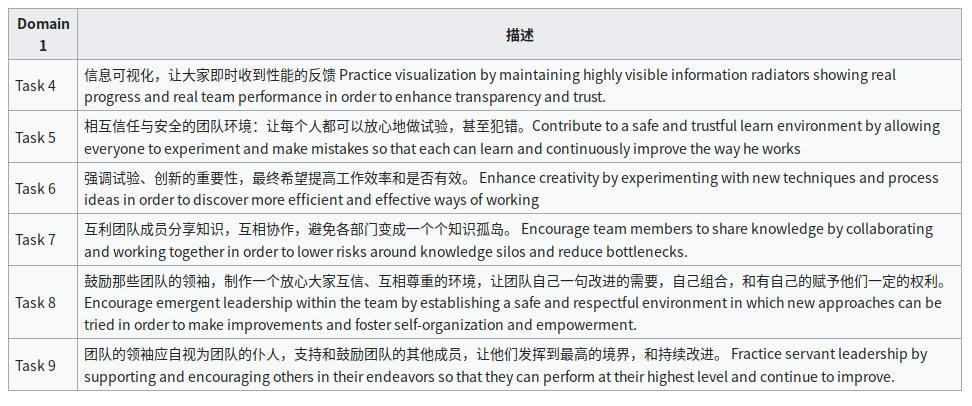
\includegraphics[width=10cm]{Screenshotfrom2022-01-23-1.jpg}

